\documentclass{article}
\usepackage{graphicx} % Required for inserting images

\title{Branched optimal transport}
\author{Antonio De Rosa, Dario Filatrella, Aida Khajavirad}
\date{August 2024}

% Packages
\usepackage{amsmath}
\usepackage{tikz-cd}
\usepackage{amsfonts}
\usepackage{amsthm}
\usepackage{amssymb}
\usepackage[
    backend=biber,
    style=alphabetic,
    sorting=ynt
]{biblatex}
\addbibresource{bib.bib}
% Document

\renewcommand\qedsymbol{$\cdot$}


\begin{document}

    \maketitle


    \tableofcontents
    \newpage


    \section{Definitions and notation}


    We will start with the most abstract definition of branched transport, which holds for generic measures $\mu^+$ and $\mu^-$.
    We will then restrict our analysis to the case where $\mu^+$ is a Dirac delta and $\mu^-$ is a finite sum of Dirac deltas.

    \subsection{Branched transport}

    This definition is taken from \cite{Bernot} and it is known as Lagrangian formulation. \\

    Given $X \subset \mathbb{R}^N$ compact and two measures of equal mass $\mu^+$ and $\mu^-$ on $X$, a traffic plan is
    a measure $P$ on $K$ that transports $\mu^+$ to $\mu^-$.
    Formally, consider the maps $\pi_0, \pi_\infty : K \rightarrow X$ given by $\pi_0(\gamma) = \gamma(0)$ and $\pi_\infty(\gamma) = \gamma(T(\gamma))$,
    $P$ is a traffic plan if:
    \[
        \mu^+ = (\pi_0)_{\#}P, \quad \mu^- = (\pi_\infty)_{\#}P
    \]

    \subsection{Parameterized Traffic Plans}
    The next paragraph is copied from the \cite{Bernot}:

    According to Skorokhod theorem (Theorem A.3 p. 185), we can parameterize any traffic plan $P$ by a measurable function
    $\chi : \Omega = [0, |\Omega|] \rightarrow K$, where $\Omega$ is a measure space which we identify with an interval, such that
    $P = \chi_{\#} \lambda$, where $\lambda$ is the Lebesgue measure on $[0, |\Omega|]$.
    We shall set $\chi(\omega, t) := \chi(\omega)(t)$ and consider it as a function of the variable pair
    $(\omega, t)$.

    With this formulation the energy (or cost) of a parameterized traffic plan is:
    \begin{equation}
        E^{\alpha}(P) = \int_{\mathbb{R}^N} |x|_P^{\alpha} d \mathcal{H}^1(x)
    \end{equation}
    There are other formulations and under some assumptions they are equivalent. In particular there should be no problem
    for finite atomic measures.

    \subsection{Euclidean Steiner Tree problem with masses}

    TODO: I am not sure how to call the case where there are masses and alpha is not 0.

    The \textbf{Euclidean Steiner Tree problem} (ESTP) is defined as follows: \\
    Given a dimension $N$, a cost parameter $\alpha$, and a set of terminal points $P = \{p_1, \ldots, p_n\}$ in $\mathbb{R}^N$ with
    corresponding masses $M = \{m_1, \ldots, m_n\}$, the goal is to find a weighted graph $(S \cup P, E, f)$, where $S = \{s_1, \ldots, s_m\}$
    consists of Steiner points $s_i \in \mathbb{R}^N$, $E \subseteq S \cup P \times S \cup P$ is the set of edges and
    $f : E \rightarrow \mathbb{R}$ is the flow on each edge.
    The graph must form a network flow with sources and sinks at the terminal points $P$ (in accordance with their masses), such that the following cost function is minimized:
    \[
        \sum_{(x,y) \in E} f_{xy}^\alpha \|x - y\|
    \]

    We are particularly interested in the case where there is a single source, so only one terminal has positive mass. In this case, the optimal solution is a tree.

    \subsection{Euclidean Steiner Tree problem}

    A special case of the ESTP is when $\alpha=0$, which implies that the cost function is the sum of the lengths of the edges, and it does not
    take into account the flow on the edges.
    In this case, masses are irrelevant and the optimal solution is a tree connecting all the terminals.
    The objective function is then:
    \begin{equation}
        \sum_{(x,y) \in E} \|x - y\|
    \end{equation}

    \subsection{Relation between ESTP and Branched transport}

    \subsubsection{Properties of branched transport}
    It is known from \cite{Bernot} that in Branched Transport the optimal solutions have a finite graph structure outside of the
    support of $\mu^+$ and $\mu^-$. In the case of finite atomic measure, this means that the optimal solution is a forest. Furthermore
    if there is only one source than it is also connected, so a tree.
    For such a graph, the cost function of a parameterized traffic plan is the same as the cost function of the ESTP if no edges with positive mass
    have intersection of positive $\mathcal{H}^1$ measure, which is the case in an optimal solution.

    From this we can deduce that the optimal solution of a Branched transport coincide with solutions to the ESTP.

    \subsubsection{Construction of an ESTP from a branched transport problem}

    We can reduce any ESTP (in the algorithmic sense) to an instance of a branched transport problem. We will give an
    explicit formulation for the single source case.

    Given a set of terminals $P = \{p^1, ..., p^{|P|}\}$ we can define:
    \begin{equation}
        \mu^+ = \delta_{p^1} \quad \mu^- = \frac{1}{|P| - 1}\sum_{i = 2}^{|P|} \delta_{p^i}
    \end{equation}
    and set $\alpha =0$ in the cost function.
    We can then use results from branched transport to say that the optimal parameterized
    traffic plan is a graph and it is loop-free. We will now prove that it is connected and conclude that it is a tree.

    For each terminal $a^i$ (with $i>1$) we have a subset $A_i \subset [0,1]$ such that $\chi(A_i)$ are all paths terminating at $a^i$ and
    $\chi(A_i)(0) = a_1$.
    We can easily conclude that every terminal is connected to $a_1$ and therefore the graph is connected.


    \section{Formulation}

    \subsection{MMX}

    \begin{align}
        \text{(MMX)}: \; \min &\sum_{[i,j] \in E_1} \|p_i - s_j\| y_{ij} + \sum_{[i,j] \in E_2} \|s_i - s_j\| y_{ij}, \\
        & \sum_{j \in S} y_{ij} = 1 \quad \text{for } i \in P, \\
        & \sum_{i \in P} y_{ij} + \sum_{k < j, k \in S} y_{kj} + \sum_{k > j, k \in S} y_{jk} = 3 \quad \text{for } j \in S, \label{MMX:connectivity_steiner} \\
        & \sum_{k < j, k \in S} y_{kj} = 1 \quad \text{for } j \in S - \{p+1\},  \\
        & y_{ij} \in \{0, 1\}, \quad [i, j] \in E, \quad s^i \in \mathbb{R}^n, \quad i \in S.
    \end{align}

    Where: \begin{itemize}
               \item $P$ is the set of terminals,
               \item $S$ is the set of Steiner points (indexed as $S = \{|P| + 1, ..., 2|P|-2\}$),
               \item $E_1$ is the set of edges connecting terminals to Steiner points,
               \item $E_2$ is the set of edges connecting Steiner points
    \end{itemize}

    \subsection{Proof of correctness}

    The MMX problem "solves" the ESTP in the sense that under certain conditions, the optimal solution of MMX corresponds to
    the optimal EST.
    Explicitly, we can construct a function $\phi$ that maps feasible solutions of MMX to feasible solutions of ESTP and such
    that the following commutative diagram holds:

    \[
        \begin{tikzcd}
            & \mathbb{R}  \\
            MMX \arrow[ur, "Obj"] \arrow[rr, "\phi"'] & & EST  \arrow[ul, "Obj"]
        \end{tikzcd}
    \]

    Where $Obj$ is the objective function of the respective problems and MMX and EST are the feasible regions.

    \subsection{Definition of $\phi$}
    The function $\phi$ maps $\mathbb{R}^{N (|P|-2)} \times \{0,1\}^{|E|}$ to a graph in $\mathbb{R}^N$ as follows:

    \begin{enumerate}
        \item For each $i \in P$, add a terminal at $p^i$.
        \item For each $j \in S$, add a vertex $v_j$ at $s^j$.
        \item For each $[i,j] \in E$ with $y_{ij} = 1$, add an edge between $v_i$ and $v_j$.
    \end{enumerate}

    There are a few issues with this identification: $\phi$ is neither injective (there is a permutation invariance in the index of both
    Steiner points and terminals) nor surjective, as for instance, the number of vertices is fixed. By an edge counting argument we know that
    the number of Steiner points in an optimal EST cannot be bigger than the ones included in MMX, but it could be lower
    (for example in the case where all terminals lie on a line).
    It is easy to see that the objective functions are the same as they both sum the Euclidean distances of the active edges.


    \textbf{Claim} Calling MMX and EST the respective feasible regions, we have that $\phi(MMX) \subseteq EST$.

    \begin{proof}
        Let $x \in MMX$ and $G = \phi(x)$. We need to show that $G$ is a tree (so connected and loop-free).
        By the first constraints, we know each terminal is connected to a Steiner point and constraint (\ref{MMX:connectivity_steiner}) ensures that
        all Steiner points are connected, so $G$ is connected.
        By edge counting, we deduce that $G$ is a tree.
    \end{proof}



    \textbf{Claim} The optimal solution of MMX is also optimal for ESTP.

    \begin{proof}
        We know that the optimal solution for the ESTP is a tree with number of vertices $|V| \le 2|P| - 2$ and degree of each vertex $d(v) \le 3$.
        We can show that for each graph with those properties there is an element in $MMX$ that maps to it.
        In $MMX$, the degree of the terminals is fixed at 1. However, we can introduce a Steiner point with the
        same coordinates as a terminal (allowing for a degenerate solution) and make the following construction for the case where $d(v) = 2$.

        We will describe a procedure to add Steiner points until a sufficient number is reached, while maintaining
        the original graph structure. Then, we will demonstrate that these operations preserve all the properties of the $MMX$ problem.

        By performing some edge counting, we observe that
        \begin{equation}
            |E| = \frac{1}{2} \left( 3|S| + \sum_{i \in P} d(i) \right)
        \end{equation}
        Which implies that:
        \begin{equation}
            \sum_{i \in P} d(i) = 2|P| - 2 - |S|
        \end{equation}
        If $|S| = 2|P| - 2$ we are done, otherwise we can find a terminal $i$ with $d(i) = 2,3$ and add 1 or 2 Steiner points respectively.
        \begin{itemize}

            \item Case $d(i) = 1 $: we add a Steiner point $s$ with connection to the two points connected to $i$ and remove the edge
            connecting $i$ to the other terminal. We also connect $s$ to the terminal $i$.

            \item Case $d(i) = 2$: Calling the points connected to $i$ $z_1, z_2, z_3$ we add two Steiner points $s_1, s_2$ and connect
            $s_1$ to $(z_1, s_2, i)$ and $s_2$ to $(s_1, z_2, z_3)$.
        \end{itemize}

        In this way we preserve connectedness, loop-freeness and the number of (non-degenerate) vertices. Connectedness implies
        \ref{MMX:connectivity_steiner} up to reordering of the Steiner points.
        We can repeat the procedure until $|S| = |P| - 2$ which is our desired number of Steiner points.
        We get that the degree of every terminal is 1 and the degree of every Steiner point is 3, so all the conditions
        of MMX are satisfied.


    \end{proof}


    \subsection{Generalized MMX}

    \subsection{Proof of correctness}


    \section{Degree problem}

    It is very useful, both practically and theoretically, to have a bound on the degree of Steiner points and terminals in the optimal solution.
    To obtain such a bound one can proceed by showing that two edges, in order to be optimal, need to have a certain angle between them. This angle can
    depend on:
    \begin{itemize}
        \item $N$: the dimension of the space
        \item $\alpha$: the parameter of the objective function
        \item $m_1, m_2$: the masses of the two edges
        \item the direction of the flow of the two edges
    \end{itemize}

    \subsection{Bounds from literature}

    For the case $N=2$ and for every $\alpha \in [0,1]$, it is known from \cite{degree3} that the degree of Steiner points and terminals is at most 3.

    From \cite{Bernot} the following lemmas can be used:

    \subsubsection{Lemma 12.2 \cite{Bernot}}

    \begin{figure}[h]
        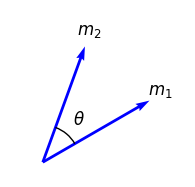
\includegraphics[scale=0.5]{angle_bound_example}
        \centering
        \caption{Picture of the bound of lemma 12.2}
    \end{figure}

    Consider a vertex $S$ and two vertices $s_1, s_2$ connected to it. Let $m_1, m_2$ be the masses of the two edges leaving
    $s$ and connecting to $p_1, p_2$ respectively.
    Let $\theta$ be the angle between the two edges. Then, for every $\alpha \in [0,1]$:
    \begin{equation}
        \cos(\theta) \le \frac{(m_1 + m_2) ^ {2\alpha} - m_1^{2\alpha} - m_2^{2\alpha}}{2m_1^\alpha m_2^\alpha}
    \end{equation}

    \subsection{Lemma 12.15 \cite{Bernot}}

    Consider a vertex $s$ and two terminals $s_1, s_2$ connected to it. Let $m_1, m_2$ be the masses of the two edges connecting
    $s$ to $s_1, s_2$ respectively. Let $\theta$ be the angle between the two edges.
    Then, for every $\alpha \in [0,1]$:

    \begin{equation}
        \cos(\theta) \le \begin{cases}
                             2^{2\alpha-1}-1 & \text{if} \frac{1}{2} < \alpha \le 1\\
                             0 & \text{if 0} \le \alpha \le \frac{1}{2}\\
        \end{cases}
    \end{equation}

    Notice that this bound is independent of the masses of the edges. In the proof of the lemma it is also proved that the function
    \begin{equation}
        f(m_1) = \frac{(1+m_1)^{2\alpha} - 1 - m_1^{2\alpha}}{2m_1^\alpha}
    \end{equation}
    is decreasing for $m_1 \in [0,1]$ and $\alpha \in [0,\frac{1}{2}]$ and increasing for $m_1 \in [0,1]$ and $\alpha \in [\frac{1}{2},1]$.

    \subsection{Improved bounds}

    \begin{figure}[h]
        \label{fig:angle_bound_example_inverted}
        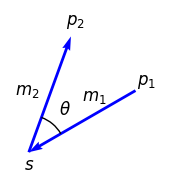
\includegraphics[scale=0.5]{angle_bound_example_inverted}
        \centering
        \caption{Picture of the bound of lemma 12.16}
    \end{figure}

    We can improve the results from the book for the case described by figure \ref{fig:angle_bound_example_inverted} TODO la ref non funziona.

    We can assume $p_1$ and $p_2$ lie on the unit circle (by zooming enough and by the property that every restriction of an optimal
    solution is optimal). Calling the candidate new branching point $x$ and setting $s=(0,0)$.
    Without loss of generality we assume $m_1 \ge m_2$. We can write the cost $f$ of this configuration of the tree as:
    \begin{equation}
        f(x) = m_1^{\alpha}\|p_1 - x \| + m_2^{\alpha} \|p_2 - x\| + (m_1-m_2)^{\alpha} \|x\|
    \end{equation}
    By setting $x = \epsilon v$ with $\|v\|=1$ and expanding to the first order around $\epsilon=0$:
    \begin{equation}
        f(\epsilon v) = f(0) - \epsilon m_1^{\alpha} v \cdot p_1 - \epsilon m_2^{\alpha} v \cdot p_2 + (m_1-m_2)^{\alpha} \epsilon + o(\epsilon)
    \end{equation}

    Given that we only want to check when $f(0)$ is not a maximum we can restrain our search around $\epsilon$ close to $0$.

    \begin{figure}[h]
        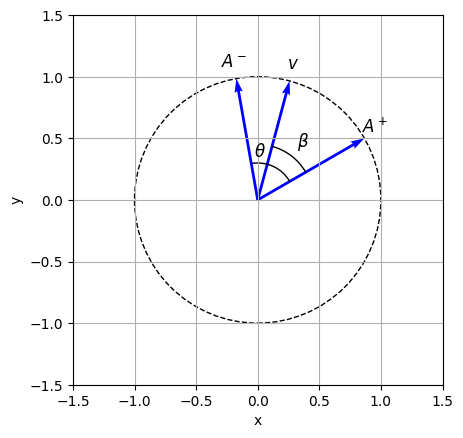
\includegraphics[scale=0.5]{circle}
        \centering
        \caption{Diagram of $p_1$, $p_2$ and $s$}
    \end{figure}

    We can parametrize $v$ with the angle $\beta$ from $p_1$ (going toward $p_2$) and get to the following equation:
    todo controlla m1 e m2 qui è asimmetrico
    \begin{equation}
        f(\epsilon) - f(0) = \epsilon \left[ (m_1-m_2)^\alpha - m_2^\alpha \cos\beta - m_1^\alpha (\cos\theta\cos\beta - \sin\theta\sin\beta) \right] + o(\epsilon)
    \end{equation}

    To prove that $\theta$ is not optimal we have two options:
    \begin{itemize}
        \item prove that there exists $\beta$ such that the first order coefficient is negative
        \item prove that the first order coefficient is bigger than $0$ for all $\beta$
    \end{itemize}


    To do this we want to fix $\theta, m_1, m_2$ and study the minimum of this function:
    \begin{equation}
    (m_1-m_2)
        ^\alpha - m_2^\alpha \cos\beta - m_1^\alpha (\cos\theta\cos\beta - \sin\theta\sin\beta)
    \end{equation}

    Calling $t = \cos(\beta)$ we get the following equations needs to have a solution for $\beta$:
    \begin{equation}
    (m_1-m_2)
        ^{\alpha} + \cos\beta(-m_2^\alpha-m_1^\alpha t) + \sin\beta(m_1^\alpha \sqrt{1-t^2}) = 0
    \end{equation}

    Having a value of $\beta$ such that the above equation evaluates to 0 is not enough, we should also check if on one side there is
    a minimum.
    We also know there is a $\beta$ such that the value is negative (take beta outside of span of $p_1, p_2$ contradicting the convex
    hull property of the optimal solution). This implies that in case of non-optimal $\theta$ this function needs to pass
    through $0$.

    todo: rendi più chiaro cosa c'è scritto qua sopra


    By solving this equation (todo check condition $c^2 \le a^2 + b^2$) we get the condition:
    \begin{equation}
        t \ge \frac{(m_1-m_2)^{2\alpha} - m_1^{2\alpha} - m_2^{2\alpha}}{2m_2^\alpha m_1^\alpha}
    \end{equation}
    Which is almost the same as lemma 12.2. There are some signs which are different so maybe I should check the computation but the
    assumptions are also slightly different (in particular one of the flows is in the other direction, which explains the $m_1-m_2$ instead
    of $m_1+m_2$).

    \subsection{Instance specific bounds}

    We now have a bound on the cosine of the angle given the masses of the two edges. Thanks to the loop-free property of the optimal solution,
    we know that the masses on the edges are combinations of masses in $M$. We can then maximize the bound of the cosine
    under this constraint to find the smallest angle that can be achieved in a specific instance of the problem. We then can
    use this angle to find a bound on the degree of the Steiner points and terminals.

    The first thing we notice is (this is useless because the rightmost term has a broader domain sadly):
    \begin{equation}
        \cos(\theta) \ge \frac{(m_1+m_2)^{2\alpha} - m_1^{2\alpha} - m_2^{2\alpha}}{2m_2^\alpha m_1^\alpha} \ge \frac{(m_1-m_2)^{2\alpha} - m_1^{2\alpha} - m_2^{2\alpha}}{2m_2^\alpha m_1^\alpha}
    \end{equation}

    \subsection{Maximizing the first bound}

    Formally for the first bound, we know both edges are flowing out so the masses are "disjoint" in the sense that there
    exist sets $A_1, A_2 \subseteq M$ such that $A_1, A_2 \neq \emptyset$, $m_1 = \sum_{i \in A_1} m_i$ and $m_2 = \sum_{i \in A_2} m_i$ and $A_1 \cap A_2 = \emptyset$.

    We first study the function for any $m_1 \in [0,1]$ and $m_2=1$, and then solve the constrained version. We can observe that there
    is a different behaviour depending on $\alpha$:
    \begin{itemize}
        \item If $\alpha \le 1/2$ we have that the function is decreasing in $m_1$. Therefore the maximum is achieved when $m_1$ is the smallest.
        \item If $\alpha > 1/2$ we have that the function is increasing in $m_1 \in [0,1]$. The maximum is achieved when $\frac{m_1}{m_2} \approx 1$.
    \end{itemize}

    \subsubsection{Case $\alpha \le 1/2$}
    In the first case, it is sufficient to take
    \begin{align}
        & m_1 = \min_{i \in M} m_i \\
        & m_2 = \sum_{i \in M} m_i - m_1
    \end{align}

    \begin{figure}[h]
        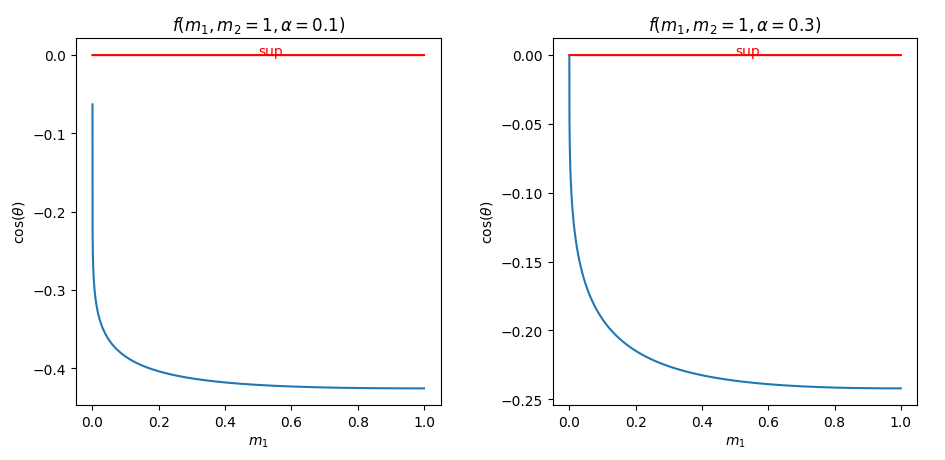
\includegraphics[scale=0.5]{f_sum_m1_m2_alpha_le_1-2}
        \centering
        \caption{Plot of the bound for $\alpha \le 1/2$}
    \end{figure}

    \subsubsection{Case $\alpha \ge 1/2$}

    The second case apears to be NP complete (this is not a justified claim). In practice we should be able to realistically bound the ratio.
    Maybe with a pigeonhole argument but it is not clear how to do it. In practice, with high probability there will be masses with ration close to 1.
    It can be seen from the graph, that even a ratio of 0.5 is already very close to the theoretical maximum.

    We need a lower bound on the distance (rather than an upper bound) so it could be more difficult to obtain one (a feasible solution is
    not enough, we need a relaxation guarantee, from the perspective of a solver), but if the upper bound is very close to the theoretical
    best (which is 0) we might just use the known sup $2^{2\alpha-1}-1$.

    \subsection{Maximizing the second bound}

    We still have to prove that the function is decreasing possa il tuono c

    \begin{figure}[h]
        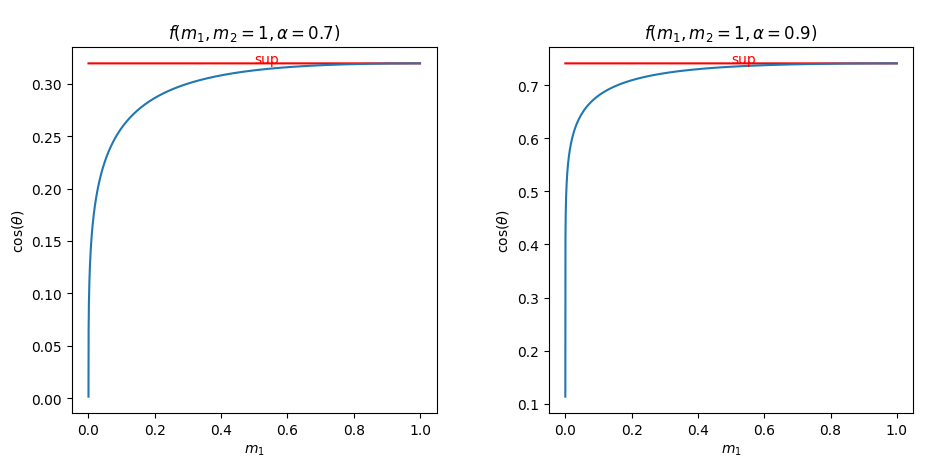
\includegraphics[scale=0.5]{f_sum_m1_m2_alpha_ge_1-2}
        \centering
        \caption{Plot of the bound for $\alpha \ge 1/2$}
    \end{figure}

    \subsection{Spherical cap results}

    \subsection{Numerical results}

    \Section{Notation}

    \subsection{Eucledian Steiner Tree problem}
    \begin{itemize}
        \item $N$: dimension of the space
        \item $\alpha \in [0,1]$: cost parameter
        \item $P = \{p_1, \ldots, p_n\}$: set of terminal points
        \item $M = \{m_1, \ldots, m_n\}$: masses of the terminal points
        \item $S = \{s_1, \ldots, s_m\}$: set of Steiner points
        \item $E$: set of edges
        \item $f_{xy}$: flow on the edge connecting $x$ to $y$
    \end{itemize}


    \newpage
    \printbibliography


\end{document}